\documentclass[conference,a4paper,twoside]{IEEEtran}

\usepackage[utf8]{inputenc}
\usepackage[T1]{fontenc}
\usepackage{flushend}
\usepackage{blindtext}
\usepackage{graphicx}
\usepackage{cite}
\usepackage[cmex10]{amsmath}
\usepackage{mathrsfs}
%\usepackage{algorithmic}
%\usepackage{array}
\usepackage{mdwmath}
\usepackage{mdwtab}
\usepackage[tight,footnotesize]{subfigure}
\usepackage[font=footnotesize]{subfig}
\usepackage{url}
\usepackage{subfigure}
\let\labelindent\relax
\usepackage{enumitem}
\usepackage{amsfonts}
\usepackage{algorithm}
\usepackage{algorithmic}

\usepackage{tikz}
\usepackage{transparent}
\usepackage{floatpag}

\usepackage{listings}
\lstset{
  frame=single,
  language=python,
  %basicstyle=\small,
}

\makeatletter
\def\lst@makecaption{%
  \def\@captype{table}%
  \@makecaption
}
\makeatother

\renewcommand{\arraystretch}{1.3}

\newcommand\given[1][]{\:#1\vert\:}

\usepackage{trackchanges}
\addeditor{mk}
\addeditor{nb}
\addeditor{mb}
\newcommand{\docite}{[Citation Needed]\note[mk]{Citation Needed}}

\begin{document}

\title{Discovering Motifs in Rodent Behaviour}

\author{
    Bachelor Thesis \\
    Marein Könings \\
    Artificial Intelligence at Radboud University \\
    Nijmegen, The Netherlands \\
    marein@science.ru.nl \\
    2017 \\
}

\maketitle
\thispagestyle{plain}
\pagestyle{plain}

\begin{abstract}
        The search for biomarkers of psychiatric disorders is an important area within translational psychiatry, as these biomarkers could potentially be transferable to humans. Research in this area involves observing behaviour of the animal under different experimental conditions (e.g. after application of a drug). Although a wide range of such experiments are conducted, there is little existing software dedicated to the analysis of the resulting data. In this work, a new method for quantifying rodent behavioural data is attempted, by applying existing research on the discovery of frequent patterns ('motifs') in time series data. These patterns are then interpreted as features to be used for classification, in order to compare the results to existing methods.
\end{abstract}

\section{Introduction}
\label{sec:intro}

\subsection{Translational psychiatry}
\label{sec:intro_transpsych}
In medical research, the term 'translation' refers to the process of transforming basic scientific research into medical applications with public impact \cite{drolet2011translational} \cite{woolf2008meaning}. Translational psychiatry, then, is the field focused on the transformation of psychiatric discoveries into medical practices and treatments \cite{machado2012tracking}. Within this field, a major area is rodent behavioural research, which looks for predictors of psychiatric disorders in animals (e.g. the amount of grooming displayed by an animal). If such so-called \emph{biomarkers} are found, new directions for research into possible treatments could be opened up. If a successful treatment for a psychiatric disorder is found in rodents, it might prove to be transferable to humans. In this way, rodent experiments have been used to study a great number of highly prevalent cognitive disorders, including schizophrenia, depression, bipolar disorder \cite{nestler2010animal}, as well as anxiety and autism \cite{stewart2015developing}.

\subsection{Open field experiments}
\label{sec:intro_openfield}
One commonly used paradigm of rodent research in translational psychiatry is the \emph{open field} experiment \cite{prut2003open}. In this type of experiment, the animal is placed in a constrained environment which they are free to explore. The behaviour of the animal is recorded and then analysed. The characteristics of the environment differ between experiments. A common setup includes a well-lit circular, square or rectangular area, bounded either by insurmountable walls or deep gaps. Often objects will be present in the environment to provoke the animal's interaction, such as platforms or tunnels. The open field paradigm is used primarily for measuring anxiety and sedation, and the reaction of a subject to a stressful situation \cite{prut2003open}.

% \begin{figure}
%     \centering
%     \begin{subfigure}{}
%         \includegraphics[width=0.45\linewidth]{images/openfield_square.png}
%     \end{subfigure}
%     \begin{subfigure}{}
%         \includegraphics[width=0.45\linewidth]{images/openfield_round.png}%
%     \end{subfigure}
%     \caption{Examples of square and circular walled open fields, from \cite{gould2009open}.}
%     \label{fig:openfield_pictures}
% \end{figure}

The animal's behaviour can be recorded in multiple ways. Commonly recorded variables include horizontal locomotion (based on a count of transitions between marked areas within the field, Figure \ref{fig:rat}), vertical activity (based on the animal's rearing and leaning behaviour) and more detailed behaviours such as grooming \cite{prut2003open}. Automated systems now to record all of the necessary variables with high precision and flexibility \cite{delcourt2006comparing}, for example by recording the animal using a video camera and processing the resulting footage with specialised software, resulting in the required variables. This setup is exemplified in Figure \ref{fig:openfield_camera}.

\begin{figure}
    \centering
    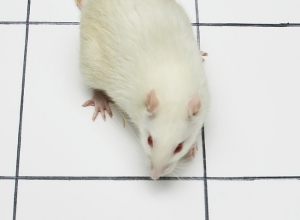
\includegraphics[width=0.45\linewidth]{images/rat.jpg}
    \caption{A rat exploring an open field, from \cite{noldus}, used with permission. This image also clearly shows the marked areas that are sometimes used to measure the animal's horizontal locomotion. \small{Image courtesy of Noldus Information Technology (www.noldus.com).}}
    \label{fig:rat}
\end{figure}

\begin{figure}
    \centering
    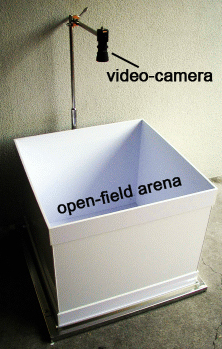
\includegraphics[width=0.45\linewidth]{images/openfield_camera.jpg}
    \caption{An example of a video tracking system, showing a square open field and a video camera in position to record the rodent's behaviour. From \cite{koide}, used with permission.}
    \label{fig:openfield_camera}
\end{figure}

Often a contrasting experimental design is used in conjuncture with the open field paradigm. In such experiments, the available animals are divided into multiple groups, with each group being treated differently in some way. Differences in observed open field behaviour between groups can then be conjectured as resulting from the difference in treatment. Common examples of differences in treatment include changes to the objects in the open field, differences in the amount of food consumption prior to the experiment, or the injection of different drugs prior to the experiment \cite{heiderstadt2000effect}.

In order to accurately describe the differences in behaviour between groups, some way to quantify the behaviour is needed. This project focuses on the creation of such a quantification method, based on some constraints and goals. The evaluation of the method happens by applying it to a given dataset of rodent behaviour in the open field.

\subsection{Text structure}
This thesis is structured as follows. First, some more background about the project is provided (Section \ref{sec:background}), followed by a description of the raw experimental data used in the project (Section \ref{sec:materials}). Then, the methods for data cleaning and preparation are described (Section \ref{sec:methods_dataprep}), followed by the methods for data augmentation (Section \ref{sec:methods_augment}). Then, the methods for the actual feature extraction are introduced (Section \ref{sec:methods_features}). The parameters of the algorithm are then described in detail (Section \ref{sec:methods_params}). Following this, a possible method for comparing the results of the given feature extraction method to other methods is presented (Section \ref{sec:methods_compare}). Next, the results of all presented methods are given (Section \ref{sec:results}). Finally, the results are discussed (Section \ref{sec:discussion}).

Note that sections \ref{sec:methods_dataprep}, \ref{sec:methods_augment}, \ref{sec:methods_compare}, \ref{sec:results_dataprep}, \ref{sec:results_augment} and \ref{sec:results_evaluate} describe work that was done in collaboration with Jesse Zwamborn.

\section{Background}
\label{sec:background}

\subsection{Quantification of rodent behaviour}
\label{sec:bg_quant}

A large number of open field experiments are performed in laboratories all over the world, yielding large amounts of behavioural data \cite{proposal}. Although software exists to extract the raw behavioural variables from video footage, little has been done to automate the further summarisation, description and analysis of the resulting data \cite{proposal}. One existing technique involves the detection of \emph{T-patterns}, which are simplified repeating sequences in the data \cite{casarrubea2015t}. However, this method can be fragile and sensitive to spurious patterns, because the it involves a large number of significance tests, increasing the risk of false positives \cite{salah2010t}. Given this gap in availability of existing software, there is an opportunity to explore new ways of quantification of rodent behaviour, in order to facilitate the interpretation of experimental results and open up new opportunities for creating behavioural biomarkers of cognitive disorders.

The goal of this project is to devise such a new method for quantifying rodent behaviour, while avoiding the shortcomings of existing methods if possible. In an attempt to formalise the construction of this new method, some definitions will be made. A \emph{quantification method} is defined in Equation \ref{eq:quant_method} as a function $Q$, mapping an animal's open field behavioural data $d$ to a sequence of numbers which should quantify its behaviour. The animal's data $d$ is an element of a dataset $D$ which contains the data from all open field recordings in a particular study. The data $d$ can have any structure, however that structure is presumed to be the same for all $d$ in $D$, and the structure is assumed to have some definable size. The resulting sequence of numbers $f_1, f_2, \dots, f_n$ is referred to as the \emph{feature vector} corresponding to the input data, because of its parallels and uses in machine learning (Section \ref{sec:methods_compare}). The length of the feature vector, and the interpretation of its elements, is constant between animals for any given quantification method.

\begin{equation} \label{eq:quant_method}
    Q(d \in D) \rightarrow \{ f_1, f_2, \dots, f_n \}
\end{equation}

To aid in finding a successful quantification method, the following sections propose some desired characteristics such a method.

\subsubsection{Conciseness}
\label{sec:bg_concise}
The conciseness of a quantification method is determined by the length of the resulting feature vector relative to the size of the input data. Since one purpose of a quantification method is compression, smaller feature vectors are preferred over larger ones. Note that the value described in Equation \ref{eq:quant_conciseness} does not depend on the choice of $d$ because of the restrictions described in the previous section.

\begin{equation} \label{eq:quant_conciseness}
    \text{conciseness}(Q) = \frac{|d|}{|Q(d)|} \text{ for any $d \in D$}
\end{equation}

\subsubsection{Accuracy}
A quantification method which yield similar features for subjects which are known to behave similarly, and dissimilar features for subjects which are known to behave dissimilarly, can be seen as highly accurate. A formal sketch of this idea is given in Equation \ref{eq:quant_accuracy}, under the assumption of an optimal method $\mathscr{Q}$. One practical way to assess the accuracy of a quantification method is through a prediction study: obtain the classification performance of a classifier trained and tested on a certain dataset, by using the features yielded by the quantification method. This technique is explored in Section \ref{sec:methods_compare}.

\begin{equation} \label{eq:quant_accuracy}
    \text{accuracy}(Q) = \frac{\Delta \mathscr{Q}(d)}{\left| \Delta \mathscr{Q}(d) - \Delta Q(d) \right|}
\end{equation}

\subsubsection{Dataset generality}
Preferably, the feature vectors produced by a quantification method are not only comparable to other feature vectors from within the initial dataset, but also to feature vectors from similar datasets in the same problem domain. In other words, the quantification method does not facilitate overfitting. Again, a practical approach to this measure employs a classifier, trained and tested respectively on two different datasets from the same domain. The beginnings of a formal definition for dataset generality are given in Equation \ref{eq:quant_general_dataset}, with elements $d$ and $e$ from some datasets $D$ and $E$ in the same problem domain and $\mathscr{Q}$ an optimal quantification method for the domain.

\begin{equation}
\label{eq:quant_general_dataset}
\begin{split}
    \Delta_\mathscr{Q} &= | \mathscr{Q}(d) - \mathscr{Q}(e) | \text{\hspace{.5em}\footnotesize(true difference)} \\
    \Delta_Q &= | Q(d) - Q(e) | \text{\hspace{.5em}\footnotesize(observed difference)} \\
    \text{generality}_\text{d}(Q) &= \frac{\Delta_\mathscr{Q}}{| \Delta_\mathscr{Q} - \Delta_Q |} \text{\hspace{.5em}\footnotesize(normalised fitness)} \\
\end{split}
\end{equation}

\subsubsection{Problem generality}
A different kind of generality that should characterise a quantification method concerns the applicability of the method to different problem domains. Some quantification methods may produce features based on a very specific behaviour displayed by the animal in the given data. Such features would not be useful when transferred to different problems where this behaviour is not relevant. An example is a behavioural feature that is based on observing the animal's anxiety - this is useful when analysing a dataset resulting from an environment where animals are anxious, but not useful in the case of a dataset which contains no signs of anxiety.

Since this characteristic is highly dependent on the nature of the problems, it is difficult to formalise. However, a practical test using classification performance is possible, given datasets from two different problem domains.

\subsubsection{Interpretability}
A quantification method which yields features that have an intuitive explanation in the original data, rather than consisting of symbols that have no obvious behavioural meaning, is highly interpretable. An example of a feature that is likely difficult to interpret would be a basis vector yielded by Principal Component Analysis \cite{wold1987principal} on a particular set of data. An easily interpretable feature would be the sinuosity of a time series - the degree to which the time series is similar to a sine function. Interpretability is an important characteristic of a quantification method, especially in a translational context such as the open field.

Unfortunately there is no obvious rigorous way to assess the interpretability of a quantification method, and it is not the purpose of this project to find one, so the relative interpretability of quantification methods will be assessed based on common sense.

\subsection{Method types}
Given these five criteria, some assessment of the space of possible quantification methods can be made. Four major types of methods are considered, as described in the next section. For each method, the four criteria as given in Section \ref{sec:bg_quant} are evaluated. A non-rigorous evaluation of the criteria is given in Table \ref{tab:feature_extraction_methods}, serving to give some indication of comparison between the methods. These evaluations are visualised in Figure \ref{fig:radial}.

\begin{table*}
    \centering
    \caption{Non-rigorous categorisation of quantification method types. }
    \begin{tabular}{ccccccc}
        Method type & Conciseness & Accuracy & Dataset Generality & Problem Generality & Interpretability & Example \\\hline
        Full data & low & high & low & high & low & N/A \\
        Mathematical descriptions & high & medium & high & medium & medium & Variable means and variances \\
        Behavioural descriptions & high & high & high & low & high & Jesse Zwamborn's project \cite{jesse} \\
        Pattern discovery & medium & high & high & high & medium & T-patterns \\
    \end{tabular}
    \label{tab:feature_extraction_methods}
\end{table*}

\begin{figure}
    \centering
    \includegraphics[width=\linewidth]{images/radar.png}
    \caption{Visualisation of the measures of quantification method characteristics as given in Table \ref{tab:feature_extraction_methods}.}
    \label{fig:radial}
\end{figure}

\subsubsection{Full data}
One trivial solution is to use the the full data as a quantification, without processing it into defined features. Although this quantification is fully accurate, the problem with this approach is the size of the feature vector, which would be equal to the length of a single session, as well as the method's propensity for overfitting and the difficulty in interpreting the features.

\subsubsection{Mathematical descriptions}
Another possibility involves a feature vector consisting of abstract mathematical descriptions of the data, for example the means and variance of the data, or slightly more involved measures such as sinuosity or spectral density. Although this results in a much shorter feature vector, as well as increasing interpretability, it becomes more difficult to create features which are also generalisable to different problems.

\subsubsection{Behavioural descriptions}
To increase interpretability, features may be based on known key behaviours of the animals rather than abstract mathematical properties \footnote{This method is featured prominently in Jesse Zwamborn's thesis \cite{jesse}.}. However, although it is quite possible to conceive of behavioural features that are suitable for a certain problem (for example involving the notion of a home base \cite{eilam1989home} or grooming behaviour in quantification of OCD) it is not certain to what extent these features will transfer to different problems, for example quantification of anxiety.

\subsubsection{Pattern discovery}
Finally, there is the option of general pattern discovery in the movement data. Although some assumptions are made about the type of data that is presented, pattern discovery methods are highly general both over datasets and over problems, at a loss of interpretability compared to more specific behavioural descriptions. Given the need for generality, this type of quantification method is the most promising, and a method of this type will be explored in this project.

\subsection{Existing pattern discovery methods}
\label{sec:bg_tpat}
Having chosen pattern discovery as the type of quantification method to explore, a suitable method of this type must be found. The previously mentioned T-pattern quantification method may be typed as pattern discovery, so it might seem suitable for application in this project. However, as also mentioned, it has some shortcomings. Some specific problems with the T-pattern method will be discussed in this section, so that the new method may avoid them.

Before extracting T-patterns, the open field is divided into a grid of zones (usually 5 by 5, Figure \ref{fig:bins}) and all instances of the subject transitioning from one zone into another are recorded. This sequence of transitions is then used by the T-pattern algorithm to discover patterns.

One issue with the T-patterns method is the apparent assumption that all areas of the open field are equally likely to be visited. In reality, the opposite is true: some areas are visited far more often than others (Figure \ref{fig:visit_dist}). The subject spends more time within these more popular zones and as such more behaviour occurs within them. However, this detailed behaviour is lost because the zones are equally spaced. At the same time, some zones are barely or never visited. A possible improvement might be a zone size based on popularity, such that all zones are visited equally often. This way, detailed behaviour can be captured, and there are no spurious, rarely visited zones.

\begin{figure}
    \centering
    \includegraphics[width=\linewidth]{images/visit_dist.png}
    \caption{Proportion of visits to each T-pattern zone in the '2014' dataset (Section \ref{sec:materials}), significantly non-uniform as per the Kolmogorov-Smirnov test ($p < 0.05$). This distribution would be uniform if the assumption made in dividing the open field into a uniform grid was correct (Section \ref{sec:bg_tpat}).}
    \label{fig:visit_dist}
\end{figure}

Another issue with the T-pattern method is the fact that zone transitions are computed with no regard to the temporal relation between crossings. That is, the time that a subject spends within a zone is of no consequence, only the order in which zones are visited counts. This is problematic as this prevents distinction between behaviours where timing is of importance (e.g. spending time near an object as opposed to just passing by it). In essence this problem is caused by the fact that the T-pattern method performs only spatial and no temporal segmentation.

Finally, the T-pattern method only uses the absolute position of the subject, and does not account for such things as objects in the open field or the animal's distance to the boundary. As such, behaviours that depend on the relative location of these features cannot be detected using T-patterns. If the location of an object changes, for example between subjects, the T-pattern method cannot discover a pattern if both subjects display the same behaviour relative to the object but in different absolute positions.

In an attempt to overcome these problems, a different quantification method, not commonly applied to rodent behaviour, will be explored in Section \ref{sec:methods_features}.

\section{Materials}
\label{sec:materials}

The Donders Institute Translational Psychiatry lab led by Dr. J. C. Glennon provided four datasets for use in this project, originating from experiments in two locations (Nijmegen and Utrecht). Each of these datasets contains data from an open field experiment on rats. Although differing in some details (Section \ref{sec:methods_dataprep}), the open field set-ups used in the experiments are the same: a walled, square area containing four small fixed objects (cubes or cylinders) to encourage exploration (Figure \ref{fig:boundary_objects}). The four datasets are referred to as the \emph{2013}, \emph{2014}, \emph{2016} and \emph{Utrecht} datasets.

\begin{figure}
    \centering
    \includegraphics[width=0.45\linewidth]{images/boundary_objects.png}
    \caption{The shape of the open field area and the positions of the four fixed objects. Note the fisheye effect visible in the shape of the boundary, caused by the video camera (Section \ref{sec:methods_dataprep_nonuniform}).}
    \label{fig:boundary_objects}
\end{figure}

As defined earlier, each dataset $D$ contains multiple data elements $d$, each from as single open field session. The same animal is recorded in multiple open field sessions, which take place days or weeks apart from each other. For example, in the \emph{2014} dataset, 12 different animals were recoreded, and each was given 13 sessions in the open field, for a total of 156 recorded sessions ($|D_{\text{2014}}| = 156$). In all datasets, animals were in the open field for 30 minutes per session (unless cut short).

All originating experiments sought to explore the effect of the psychoactive drug \emph{quinpirole} on the behaviour of rats, specifically its effect on biomarkers of obsessive-compulsive disorder (OCD). OCD is a mental disorder characterised by intrusive repetitive thoughts and behaviours \cite{stein2002obsessive}, and quinpirole has been already been reported to induce behaviours associated with OCD in rats \cite{szechtman1998quinpirole}. To this end, within each dataset, the animals are divided into at least two groups based on a contrasting design. Prior to some or all open field sessions, the animal received an injection based on their group assignment. In most datasets, the animal either received an injection containing quinpirole or a placebo injection containing only saline (salt water). One dataset additionally contains a third group, in which animals received an injection containing \emph{memantine}, an NMDA receptor antagonist that is associated with reduction in OCD behaviour \cite{grados2015selective}.

The animal's behaviour in the open field was recorded by an overhead video camera as described in Section \ref{sec:intro_openfield}. The resulting footage was then processed by the video tracking system Ethovision from Noldus IT \cite{noldus2001ethovision}, which produced multiple time series for each 30-minute session, representing different variables describing the raw data (Table \ref{tab:variables}). The set of available variables is represented here by $V$. The collection of time series resulting from processing a session's video footage corresponds to a single $d$ in $D$ (Equation \ref{eq:datavars}). Some visualisations of parts of the data can be found in Figure \ref{fig:plot_xy}.

\begin{equation}\label{eq:datavars}
    d \in D = \{ d_v \given v \in V \}
\end{equation}

\begin{table*}[!t]
        \caption{Descriptions of variables contained in the data.}
        \label{tab:variables}
        \centering
        \begin{tabular}{ccl}
                Variable & Unit & Description \\
                \hline
                Trial time & seconds & time since the animal was introduced into the open field environment \\
                Recording time & seconds & time since the video recording was started \\
                X centre & centimetres & x-coordinate of the animal's centre \\
                Y centre & centimetres & y-coordinate of the animal's centre \\
                X nose & centimetres & x-coordinate of the animal's nose \\
                Y nose & centimetres & y-coordinate of the animal's nose \\
                X tail & centimetres & x-coordinate of the animal's tail \\
                Y tail & centimetres & y-coordinate of the animal's tail \\
                Area & square centimetres & the amount of area covered by the body of the animal \\
                Areachange & square centimetres & the amount of body area that does not overlap with the body area of the previous measurement \cite{juszczak2008computer} \\
                Elongation & & a measure of how much the animal stretches its body out, between 0 and 1 \\
                Direction & degrees & the direction the animal is facing \\
        \end{tabular}
\end{table*}

\begin{figure}
    \centering
    \begin{subfigure}{}
        \includegraphics[width=\linewidth]{images/plot_xy.png}
    \end{subfigure}
    \hfill
    \begin{subfigure}{}
        \includegraphics[width=0.45\linewidth]{images/plot_2d.png}
    \end{subfigure}
    \begin{subfigure}{}
        \includegraphics[width=0.45\linewidth]{images/plot_2db.png}
    \end{subfigure}
    \caption{Plots showing the movement of a rat (X centre and Y centre variables) in a single session over time and through space. All data is from the \emph{2014} dataset. The lower left spatial plot corresponds to the temporal plot above (rat 109, session 4). The lower right plot originates from rat 113, session 1.}
    \label{fig:plot_xy}
\end{figure}

\section{Methods}
\label{sec:methods}

\subsection{Data preparation}
\label{sec:methods_dataprep}
It was found that the experimental data contained missing values, non-uniform structure, redundancy and anomalous data. For each of these problems, a solution is proposed in the following sections. Most solutions involve disregarding parts of the original data, but enough data remains to support the aim of the project, especially after augmentation (Section \ref{sec:methods_augment}).

\subsubsection{Missing values}
\label{sec:methods_dataprep_missing}
The available datasets were incomplete in multiple ways. Firstly, some sessions were completely missing. Secondly, some sessions were cut short, presumably as a result of problems occurring during the experiment. Lastly, some data was missing within experiments, leading to long contiguous periods missing data within a session. Specifically, some gaps have a spatial nature: they recur in multiple sessions, always at the same area in space (Figure \ref{fig:gap}). In sessions affected by these kinds of gaps, whenever the subject passes through the affected area, a temporal gap in the data occurs. Since the spatial form of these gaps is roughly elliptical, these kinds of gaps are most likely caused by shadows or highlights on the surface of the open field. These features are thought to be problematic for the computer vision software determining the subject's position, causing the missing values as seen. The effect is less prominent in the \emph{X centre} and \emph{Y centre} variables, with most missing values occurring in the other \emph{X} and \emph{Y} variables.

\begin{figure}
    \centering
    \begin{subfigure}{}
        \includegraphics[width=0.45\linewidth]{images/singlegap.png}
    \end{subfigure}
    \begin{subfigure}{}
        \includegraphics[width=0.45\linewidth]{images/gap.png}
    \end{subfigure}
    \caption{The two images illustrate the issue of missing values that have a spatial nature. The image on the left shows a single session from the \emph{2013} dataset (rat 32, week 2) that suffers from the problem. A large area to the centre left of the open field is devoid of paths. All encroaching paths are cut off at the boundary of the area. The image on the right shows an overlay of all sessions in week 2 from the \emph{2013} dataset, with each animal a different colour. The gap, although less pronounced, is also visible here, showing that it is a structural problem.}
    \label{fig:gap}
\end{figure}

Multiple solutions to these problems were considered, most prominently either generation of new data to fill the gaps or complete removal of sessions containing missing data. It was determined that generation of new data was a difficult problem, especially considering that this would require prior characterisation of the existing data, while characterisation is just the point of the project. Hence it was decided to remove all sessions containing any missing data. The focus of the project was also put on those variables which contain the least missing values.

\subsubsection{Non-uniformity}
\label{sec:methods_dataprep_nonuniform}

The data displayed problematic non-uniformity between and within datasets, causing problems when comparing data points. For example, the scale and orientation of the coordinate space might differ between datasets. These problems can largely be attributed to differences in camera position and angle at the time of recording. Because of perspective and lens distortion effects, these camera parameters have a large effect on the shape of the open field as projected into two-dimensional space. Although within any single session the camera is stationary, these effects cause problems when attempting to compare between sessions and datasets where the camera parameters differ (Figure \ref{fig:overlay}). For this reason, only a single dataset is used for the project, namely the dataset which contains the largest number of sessions, and also happens to display uniform camera parameters between sessions.

\begin{figure}
    \centering
    \includegraphics[width=\linewidth]{images/overlay.png}
    \caption{An overlay of all movement data for all sessions from datasets \emph{2013} and \emph{2014}. Although the locations of objects and boundaries are aligned between sessions within datasets, there is a clear difference in these locations between datasets, as can be seen by the displacement effect in the image. The projections from the two datasets have been translated and rotated to achieve a best fit, but even so the difference is clear.}
    \label{fig:overlay}
\end{figure}

An additional problem is caused by the fisheye effect that is visible in many figures in this text, for example Figure \ref{fig:boundary_objects}. An almost unpreventable effect of using a video camera, it causes the recorded footage to become warped. Since the analysis software Ethovision does not take this issue into account, the resulting data is also warped. Although the severity of the effect on further data analysis is not obvious, it would be good to try and revert the warping effect in the resulting data. However, that has not been attempted in this project.

\subsubsection{Anomalies}
Throughout the sessions, some anomalous data can be found, which take the form of sudden jumps seemingly made by the subject over large distances from one location to another (the 'teleportation effect'). Sometimes these anomalies even seem to transport the subject to locations outside the regular bounds of the open field (for example Figure \ref{fig:gap}). These jumps almost always come in pairs, where the subject is transported to an anomalous location and then transported back to the original area after a fraction of a second. It seems that these anomalies can be attributed to errors made by the computer vision software when extracting the movement data from the raw video footage. Anomalies may be detected by looking for position deltas between two adjacent time points that would be impossible for an actual rat to accomplish. Assuming a top speed of 9.6 km/h for rats \cite{wolfram}, 93 such deltas occur in the \emph{2014} dataset (0.002\% of all time points), an order of magnitude less than the \emph{2013} dataset.

One elegant solution to the problem of anomalies would be to detect the anomalies, remove the data between two instances of 'teleportation' so that the period of anomalous movement is no longer present, and then reconstruct the missing values. However, as discussed in Section \ref{sec:methods_dataprep_missing}, the generation of new data is its own difficult problem. It was chosen that the problem of anomalous data be ignored because only such a small percentage of all data is affected.

\subsubsection{Redundancy}
Since the original data contains a large number of variables, some of which describe phenomena that seem closely intertwined, it was speculated that there was a large amount of redundancy in the data. For example, the location of the subject's head should be largely predictable from the location of the subject's torso. If this is the case, it might be possible to remove certain variables from the data, without losing any descriptive power with regards to the final features.

To investigate this thoroughly, the pairwise correlations between all of the variables in the complete dataset \footnote{That is, what is left of the dataset after previous pruning steps.} are computed, yielding measures of the extent to which each variable could be predicted from each of the others. Additionally, the statistical significance is determined, in order to support its validity.

To calculate the correlation of any two variables $v,w \in V$, Pearson's $r(v,w)$ was used, after which the incomplete beta function was used to estimate the significance $p(v,w)$ \cite{scipypearson}.

Given these, we may define the notion of a significantly, highly correlating pair of variables $v$ and $w$, given some threshold correlation $\dot{r}$ and threshold $p$-value $\dot{p}$ (0.95 and 0.05 were used respectively in this case), as formalised by the boolean function $R$ in Equation \ref{eq:sigcorvars}.

\begin{equation}\label{eq:sigcorvars}
    R(v,w) = r(v,w) \geq \dot{r} \text{ and } p(v,w) \leq \dot{p}
\end{equation}

Going further, the set of variables can be pruned so that only those variables remain which do not significantly, highly correlate with any earlier variable. Given two variables $v,w \in V$, the variable $w$ is 'earlier' than $v$ ($w<v$) if $w$ precedes $v$ in the standard order of variables as used in Section \ref{sec:materials}. The resulting set of variables $V'$ is defined in Equation \ref{eq:prunedvariables}.

\begin{equation}\label{eq:prunedvariables}
    \begin{split}
        V' = \{ v \in V \given & \neg \exists_{w \in V} w < v \text{ and } R(v,w) \}
    \end{split}
\end{equation}

This pruning technique ensures that out of all sets of inter-correlating variables, only one remains, namely the first in the order as defined.

\subsection{Data augmentation}
\label{sec:methods_augment}

Given the ultimate intent of creating a quantification method and evaluating it using classification, it is important to have sufficient data points for effectively training a classifier. Since the data undergoes significant reduction as part of the methods described in Section \ref{sec:methods_dataprep}, the possibility of data augmentation was considered. In machine learning, data augmentation is the process of extending the available data to be more multitudinal or vibrant, before using it as input for learning algorithms \cite{fawzi2016adaptive}.

Several approaches exist to data augmentation. One commonly used method involves the creation of new data with the same characteristics as the original. However, as noted in Section \ref{sec:methods_dataprep_missing}, generating synthetic open field data would require research of a scope that is beyond the current project. Instead, an approach is used that extract more data points from the available data.

Given that each session is reduced to a single data point (set of features), the amount of data points is equal to the amount of sessions. However, the fact that each session is half an hour in length can be exploited, since the features which indicate the class of a session may be observable within far less than half an hour. Thus, perhaps it is valid to split each session into a number of segments, which can then all be used for feature extraction, yielding a larger number of data points than before.

It it not obvious what is the right number of segments to split each session into. Intuitively it seems clear that if the sessions are split into too many segments, each segment will be so small that all features are lost. However, the smaller the segments are, the more data points are yielded. Thus, there is a trade-off between the length of the data in each segment, and the number of segments (Figure \ref{fig:tradeoff}).

\begin{figure}
    \centering
    \includegraphics[width=0.45\linewidth]{images/tradeoff.png}
    \caption{A visualisation of the trade-off between the length of the data in each segment, and the number of segments. Compare with the images in Figure \ref{fig:plot_xy}, which definitely lend themselves to making some statement about the behaviour of the animal, whereas the above image (showing a very small segment of an open field session) simply has too little features to use for describing behaviour.}
    \label{fig:tradeoff}
\end{figure}

Two methods for determining the optimal segment size are evaluated. The first method is based on the variance of the data in a segment as the segment size changes. As the segment size decreases, the variance in the data must decrease also. The significance of this decrease from the original can be calculated, and based on this a segment size can be chosen that is as small as possible while not displaying a significant difference in variance from the original size.

The second method for determining the optimal segment size makes use of existing literature. Many rodent experiments involve measuring the frequency of certain behaviours displayed by the animal, such as grooming or marble-burying. If the frequency of such behaviours can be determined from the literature, especially with regards to OCD behaviour, then this would be a good indication of how small segments can be while retaining the possibility to detect these behaviours in each segment.

\subsection{Quantification method}
\label{sec:methods_features}

Once data has been prepared and augmented, the feature extraction process can be started. An existing method, $k$-motifs, is employed to find recurring patterns in the data. This method involves two algorithms: Symbolic Aggregate Approximation (SAX) and Sequitur grammar induction. Although $k$-motifs successfully yields frequent patterns from a time series, it does not create feature vectors that can be used to compare multiple time series, so a conversion strategy must be devised. Additionally, while patterns in raw movement data are useful, even more patterns may be found by exploiting the animal's position relative to different aspects of the open field. Finally, $k$-motifs produces a very large amount of patterns, so to ensure the conciseness of the quantification method (Section \ref{sec:bg_concise}), some subset of these must be selected to be uses in the final feature vector. A schematic representation of the full quantification method is given in Figure \ref{fig:schema}. All of these topics will be discussed in the following sections.

\begin{figure*}
    \centering
    \begin{tikzpicture}[scale=0.95]

    \draw[rounded corners=15pt, thick, double distance=3pt, color=gray!50]
        (-7,-11.25) rectangle ++(4.75,-10.25);


    \node at (0,0)
        {\includegraphics[width=.05\textwidth]{images/plot_2d.png}};
    \node at (1,0)
        {\includegraphics[width=.05\textwidth]{images/plot_2d.png}};
    \node at (2,0)
        {\includegraphics[width=.05\textwidth]{images/plot_2d.png}};
    \node at (3,0)
        {{\transparent{0.66}\includegraphics[width=.05\textwidth]{images/plot_2d.png}}};
    \node at (4,0)
        {{\transparent{0.33}\includegraphics[width=.05\textwidth]{images/plot_2d.png}}};
    \draw (-0.6,-0.6) -- (4.6,-0.6) -- (4.6,0.6) -- (-0.6,0.6) -- (-0.6,-0.6);
    \draw[dashed] (-0.5,-0.5) -- (0.5,-0.5) -- (0.5,0.5) -- (-0.5,0.5) -- (-0.5,-0.5);

    \draw[dashed] (-4.5,1.5) -- (-0.5,0.5);
    \draw[dashed] (-4.5,-1.5) -- (-0.5,-0.5);
    \node at (-3,0)
        {\includegraphics[width=.15\textwidth]{images/plot_2d.png}};
    \draw[dashed] (-4.5,-1.5) -- (-4.5,1.5) -- (-1.5,1.5) -- (-1.5,-1.5) -- (-4.5,-1.5);
    \draw[dashed] (-1.5,1.5) -- (0.5,0.5);
    \draw[dashed] (-1.5,-1.5) -- (0.5,-0.5);

    \node[draw] at (2,1.1) {dataset $D$};
    \node[draw] at (-3,2.1) {data point $d$};

    \draw [line width=1.5] (5.5,0) circle [radius=0.3] node {1};

    \node at (0,-3)
        {\includegraphics[width=.05\textwidth]{images/plot_2d.png}};
    \node at (1,-3)
        {\includegraphics[width=.05\textwidth]{images/plot_2d.png}};
    \node at (2,-3)
        {\includegraphics[width=.05\textwidth]{images/plot_2d.png}};
    \node at (3,-3)
        {{\transparent{0.66}\includegraphics[width=.05\textwidth]{images/plot_2d.png}}};
    \node at (4,-3)
        {{\transparent{0.33}\includegraphics[width=.05\textwidth]{images/plot_2d.png}}};

    \node at (0,-4)
        {\includegraphics[width=.05\textwidth]{images/plot_2d_r.png}};
    \node at (1,-4)
        {\includegraphics[width=.05\textwidth]{images/plot_2d_r.png}};
    \node at (2,-4)
        {\includegraphics[width=.05\textwidth]{images/plot_2d_r.png}};
    \node at (3,-4)
        {{\transparent{0.66}\includegraphics[width=.05\textwidth]{images/plot_2d_r.png}}};
    \node at (4,-4)
        {{\transparent{0.33}\includegraphics[width=.05\textwidth]{images/plot_2d_r.png}}};

    \node at (0,-5)
        {\includegraphics[width=.05\textwidth]{images/plot_2d_g.png}};
    \node at (1,-5)
        {\includegraphics[width=.05\textwidth]{images/plot_2d_g.png}};
    \node at (2,-5)
        {\includegraphics[width=.05\textwidth]{images/plot_2d_g.png}};
    \node at (3,-5)
        {{\transparent{0.66}\includegraphics[width=.05\textwidth]{images/plot_2d_g.png}}};
    \node at (4,-5)
        {{\transparent{0.33}\includegraphics[width=.05\textwidth]{images/plot_2d_g.png}}};

    \node at (0,-6)
        {\includegraphics[width=.05\textwidth]{images/plot_2d_p.png}};
    \node at (1,-6)
        {\includegraphics[width=.05\textwidth]{images/plot_2d_p.png}};
    \node at (2,-6)
        {\includegraphics[width=.05\textwidth]{images/plot_2d_p.png}};
    \node at (3,-6)
        {{\transparent{0.66}\includegraphics[width=.05\textwidth]{images/plot_2d_p.png}}};
    \node at (4,-6)
        {{\transparent{0.33}\includegraphics[width=.05\textwidth]{images/plot_2d_p.png}}};

        \draw (-0.6,-6.6) -- (4.6,-6.6) -- (4.6,-2.4) -- (-0.6,-2.4) -- (-0.6,-6.6);
        \draw[dashed] (-0.5,-0.5) -- (0.5,-0.5) -- (0.5,0.5) -- (-0.5,0.5) -- (-0.5,-0.5);

        \node[draw] at (2,-1.9) {spatial relations};
        \draw [line width=1.5] (5.5,-4.5) circle [radius=0.3] node {2};

        \draw[->,thick,double distance=2.0pt] (2,-0.7) -- (2,-1.5);
        \draw[->,thick,double distance=2.0pt] (-0.7,-4.5) -- (-2.2,-4.5);

        \draw (-6,-1.5) edge[out=260,in=180,looseness=1,->,thick] (-4.1,-2.25);
        \draw [line width=1.5] (-6.5,-4.5) circle [radius=0.3] node {3};
        \node[draw,fill=white] at (-4.1,-2.25) {SAX bins};

        \draw [line width=0, draw=gray!50, fill=gray!25] (-6,-1.5) circle [radius=0.3] node {$\alpha$};

        \node at (-5,-3.5)
            {\includegraphics[width=.1\textwidth]{images/absposbins_b.png}};
        \node at (-3.2,-3.5)
            {\includegraphics[width=.1\textwidth]{images/absposbins.png}};
        \node at (-3.2,-5.3)
            {\includegraphics[width=.1\textwidth]{images/absposbins_g.png}};
        \node at (-5,-5.3)
            {\includegraphics[width=.1\textwidth]{images/absposbins_p.png}};

        % CLASSES

        \node at (-4.5,-9)
            {\includegraphics[width=.025\textwidth]{images/plot_2d.png}};
        \node at (-4,-9)
            {{\transparent{0.66}\includegraphics[width=.025\textwidth]{images/plot_2d.png}}};
        \node at (-3.5,-9)
            {{\transparent{0.33}\includegraphics[width=.025\textwidth]{images/plot_2d.png}}};
        \node at (-4.5,-9.5)
            {\includegraphics[width=.025\textwidth]{images/plot_2d_r.png}};
        \node at (-4,-9.5)
            {{\transparent{0.66}\includegraphics[width=.025\textwidth]{images/plot_2d_r.png}}};
        \node at (-3.5,-9.5)
            {{\transparent{0.33}\includegraphics[width=.025\textwidth]{images/plot_2d_r.png}}};
        \node at (-4.5,-10)
            {\includegraphics[width=.025\textwidth]{images/plot_2d_g.png}};
        \node at (-4,-10)
            {{\transparent{0.66}\includegraphics[width=.025\textwidth]{images/plot_2d_g.png}}};
        \node at (-3.5,-10)
            {{\transparent{0.33}\includegraphics[width=.025\textwidth]{images/plot_2d_g.png}}};
        \node at (-4.5,-10.5)
            {\includegraphics[width=.025\textwidth]{images/plot_2d_p.png}};
        \node at (-4,-10.5)
            {{\transparent{0.66}\includegraphics[width=.025\textwidth]{images/plot_2d_p.png}}};
        \node at (-3.5,-10.5)
            {{\transparent{0.33}\includegraphics[width=.025\textwidth]{images/plot_2d_p.png}}};

        \draw (-4.8,-8.7) -- (-3.2,-8.7) -- (-3.2,-10.8) -- (-4.8,-10.8) -- (-4.8,-8.7);

        \node at (4.5,-9)
            {{\transparent{0.33}\includegraphics[width=.025\textwidth]{images/plot_2d.png}}};
        \node at (4,-9)
            {{\transparent{0.66}\includegraphics[width=.025\textwidth]{images/plot_2d.png}}};
        \node at (3.5,-9)
            {{\transparent{1}\includegraphics[width=.025\textwidth]{images/plot_2d.png}}};
        \node at (4.5,-9.5)
            {{\transparent{0.33}\includegraphics[width=.025\textwidth]{images/plot_2d_r.png}}};
        \node at (4,-9.5)
            {{\transparent{0.66}\includegraphics[width=.025\textwidth]{images/plot_2d_r.png}}};
        \node at (3.5,-9.5)
            {{\transparent{1}\includegraphics[width=.025\textwidth]{images/plot_2d_r.png}}};
        \node at (4.5,-10)
            {{\transparent{0.33}\includegraphics[width=.025\textwidth]{images/plot_2d_g.png}}};
        \node at (4,-10)
            {{\transparent{0.66}\includegraphics[width=.025\textwidth]{images/plot_2d_g.png}}};
        \node at (3.5,-10)
            {{\transparent{1}\includegraphics[width=.025\textwidth]{images/plot_2d_g.png}}};
        \node at (4.5,-10.5)
            {{\transparent{0.33}\includegraphics[width=.025\textwidth]{images/plot_2d_p.png}}};
        \node at (4,-10.5)
            {{\transparent{0.66}\includegraphics[width=.025\textwidth]{images/plot_2d_p.png}}};
        \node at (3.5,-10.5)
            {{\transparent{1}\includegraphics[width=.025\textwidth]{images/plot_2d_p.png}}};

        \draw (4.8,-8.7) -- (3.2,-8.7) -- (3.2,-10.8) -- (4.8,-10.8) -- (4.8,-8.7);

        \draw[->,thick,double distance=2.0pt] (2,-6.7) -- (3,-8);
        \draw[->,thick,double distance=2.0pt] (2,-6.7) -- (-3,-8);

        \node[draw] at (-4,-8.3) {class 1};
        \node[draw] at (4,-8.3) {class 2};

        \draw [line width=1.5] (1.75,-7.5) circle [radius=0.3] node {4};


        \node at (-4,-12.5)
            {\includegraphics[width=0.15\textwidth]{images/presax.png}};

        \node at (-4,-15.2)
            {\includegraphics[width=0.15\textwidth]{images/postsax.png}};

        \draw[->,thick,double distance=2.0pt] (2,-0.7) -- (2,-1.5);

        \draw[dashed] (-4.25,-10.75) -- (-4.25,-10.25) -- (-3.75,-10.25) -- (-3.75,-10.75) -- (-4.25,-10.75);

        \draw[dashed] (-4.25,-10.75) -- (-5.4,-11.6);
        \draw[dashed] (-3.75,-10.75) -- (-2.6,-11.6);


        \draw (-6,-14) edge[out=40,in=180,looseness=1,->,thick] (-4,-13.8);
        \draw (-5.7,-6) edge[out=270,in=180,looseness=1.2,->,thick] (-4,-13.8);
        \draw[->,thick,double distance=2.0pt] (-4,-13.45) -- (-4,-14.25);
        \node[draw,fill=white] at (-4,-13.8) {SAX};
        \draw [line width=0, draw=gray!50, fill=gray!25] (-6,-14) circle [radius=0.3] node {$w$};

        \draw [line width=1.5] (-6.25,-15.2)circle [radius=0.3] node {5};

        \node at (-4,-17.9)
            {\includegraphics[width=0.15\textwidth]{images/seq.png}};

        \draw[->,thick,double distance=2.0pt] (-4,-16.15) -- (-4,-16.95);
        \node[draw,fill=white] at (-4,-16.5) {Sequitur};

        \draw[->,thick,double distance=2.0pt] (-4,-18.85) -- (-4,-19.65);
        \node[draw,fill=white] at (-4,-19.2) {Motifs};

        \node[draw,draw=none,fill=white] at (-4,-20) {$a\ b\ c\ a\ b\ d$};
        \node[draw,draw=none,fill=white] at (-4,-20.5) {$a\ b$};
        \node[draw,draw=none,fill=white] at (-4,-21) {$\cdots$};

        \node[draw,align=center] at (0,-13.8) {\footnotesize $a\ a\ c\ b\ b$ \\ \footnotesize $b\ b$ \\ \footnotesize $a\ a\ b\ a$ \\ \footnotesize $a\ b\ a\ a$ \\ \footnotesize $c\ c$ \\ \footnotesize $\cdots$};
        \draw (-3,-20.5) edge[out=0,in=180,looseness=.75,->,thick, double distance=2.0pt] (-0.75,-13.8);

        \draw (-1.75,-11) edge[out=260,in=180,looseness=1,->,thick] (0,-12) ;
        \draw (-1,-10.75) edge[out=260,in=180,looseness=1,->,thick] (0,-12) ;
        \node[draw,fill=white,align=center] at (0,-12) {interesting \\ class 1 motifs};

        \draw [line width=1.5] (-1.5,-12.9) circle [radius=0.3] node {6};

        \draw [line width=0, draw=gray!50, fill=gray!25] (-1.75,-11) circle [radius=0.3] node {$I$};
        \draw [line width=0, draw=gray!50, fill=gray!25] (-1,-10.75) circle [radius=0.3] node {$k$};


        \node[draw,align=center] at (3.5,-13.8) {\footnotesize $a\ c\ c\ d\ c$ \\ \footnotesize $d\ b\ d$ \\ \footnotesize $c\ a$ \\ \footnotesize $c\ a\ a\ b$ \\ \footnotesize $d\ c\ b$ \\ \footnotesize $\cdots$};
        \node[draw,fill=white,align=center] at (3.5,-12) {interesting \\ class 2 motifs};

        \draw[->,thick,double distance=2.0pt] (3.75,-10.9) -- (3.5,-11.5);

        \node at (1.75,-17.5)
            {\includegraphics[width=0.15\textwidth]{images/motifscrop.png}};

        \draw[->,thick,double distance=2.0pt] (0.25,-15.1) -- (0.5,-15.8);
        \draw[->,thick,double distance=2.0pt] (3.25,-15.1) -- (3,-15.8);

        \node[draw,fill=white,align=center] at (1.75,-15.5) {combine};
        \draw [line width=1.5] (1.75,-14.75) circle [radius=0.3] node {7};

        \node[draw,fill=white,align=center] at (4.5,-17.4){data point};
        \node at (4.5,-18.5)
            {\includegraphics[width=.075\textwidth]{images/plot_2d.png}};

        \node[draw,fill=white,align=center] at(1.75,-20.5) {\tiny $29\ 22\ 5\ 19\  5\ 21\  2\ 21\ 17\ 16\ 22\ 29\ 19\ 21\ 21\ 17\ 13\ 18\ 17\ 20$};

        \node[draw,fill=white,align=center] at (1.75,-21.1) {feature vector};

        \draw (4.5,-19.25) edge[out=-90,in=90,looseness=.75,->,thick, double distance=2.0pt] (1.75,-20.2);
        \draw[->,thick,double distance=2.0pt] (1.75,-19.1) -- (1.75,-20.2);
        \draw [line width=1.5] (1,-19.6) circle [radius=0.3] node {8};

        \node[draw=none,fill=white,align=center,text=gray!50] at (-6,-21.1) {$k$-motifs};

    \end{tikzpicture}
    \caption{Schematic visualisation of the new quantification method based on $k$-motifs. The process starts with the supplied dataset (1), containing movement data from multiple open field sessions. Each of these sessions is then transformed into multiple spatial relations (2). For each spatial relation, the SAX bins are computed, using the parameter $\alpha$ (3). The spatial relations are then separated based on the class of the session (4). For each class, every data point is processed using $k$-motifs, using the parameter $w$ and the SAX bins computed earlier (5). For each data point, this results in a set of motifs, and all motifs of a class are gathered into a list. The motifs are sorted according to some measure of interest, which is parameterised as $I$, and then some amount, parameterised as $k$, of top motifs is chosen to represent the class (6). The top motifs from each class are then combined to create the final set of motifs (7). These can then be used to create a feature vector for any data point (from the original data or otherwise), by counting the amount of times each motif occurs in the data point (8).}
    \label{fig:schema}
    \thisfloatpagestyle{empty}
\end{figure*}

\subsubsection{$k$-motifs}
In an effort to address the problems with T-patterns, a different pattern discovery algorithm was sought. After exploring several potential methods, a method was selected that seemed the most suitable and promising for the open field data data quantification problem. This method, called $k$-motifs, efficiently detects and describes recurring patterns in time series data \cite{lonardi2002finding} \cite{li2010approximate}.

It does so in two parts. The first part, Symbolic Aggregate Approximation (SAX), segments the data both in the temporal domain and in the value domain. The second part, grammar induction using Sequitur, finds patterns in the resulting approximation by constructing a hierarchical grammar. These parts are covered individually in the following sections.

\subsubsection{Symbolic Aggregate Approximation (SAX)}
The SAX algorithm takes a real-valued time series $x$ and discretises it \cite{lin2003symbolic}, starting by slicing the values into segments of size $w$. For each segment, the values contained within are averaged. This results in a new time series $t$ of length $\frac{|x|}{w}$. Next, the range of the values is divided into a number $\alpha$ of bins which are represented by the lowest value in the bin. Additionally, the bins are given unique identifiers (in this text they are numbered 0 through $\alpha-1$ using the ordering of the bins). Then, each value in $t$ is replaced by the identifier of the bin to which is belongs - that is, the highest bin whose lowest value is lower than the given value in $t$. The result is an approximate symbolic representation of the original time series. This transformation is formalised in Equation \ref{eg:sax}. An example segmentation can be seen in Figure \ref{fig:sax}.

\begin{equation}
\begin{split}
    \text{SAX}(x,w,bins) = \Big[ i \text{ for } p \text{ in } \big[ 0, 1, \cdots, \frac{|x|}{w} - 1 \big] \text{ s.t. } \\
    bins_i \leq \Sigma_{pw \leq j < (p+1)w} \frac{x_j}{w} < bins_{i+1} \Big]
\end{split}
\label{eg:sax}
\end{equation}

\begin{figure*}
    \centering
    \includegraphics[width=\linewidth]{images/mysax.png}
    \caption{A visualisation of the SAX algorithm. The real-valued input data is shown in black, which may be a near-continuous sequence. In this example, $w$ is such that the input is divided into segments of $1.2$ time units. The mean of the data in each segment is taken to produce the approximation sequence, shown in green. Finally, for each mean the corresponding bin is determined. In this example, there are four bins ($\alpha = 4$) shown to the right and delineated using dotted red lines. The normalising nature of the bin distribution can be observed. The final output in this example is $2\ 0\ 3\ 1\ 2$.}
    \label{fig:sax}
\end{figure*}

% \begin{algorithm}
%     \caption{SAX}
%     \begin{algorithmic}[1]
%         \renewcommand{\algorithmicrequire}{\textbf{Input:}}
%         \renewcommand{\algorithmicensure}{\textbf{Output:}}
%         \REQUIRE $x$, $w$, $bins$
%         \ENSURE  aggregate symbolic approximation of $x$
%         \STATE $segments$ $\gets$ split $x$ into parts of size $w$
%         \STATE $means$ $\gets$ mean of each part in $segments$
%         \STATE $digits$ $\gets$ index in $bins$ of each mean in $means$
%         \RETURN $digits$
%     \end{algorithmic}
% \end{algorithm}

Note that if $x$ is not divisible by $w$, $x$ is padded with the last value of $x$ until it is divisible by $w$.

The bins that are used to divide the value range are chosen as percentiles of a normal distribution with mean and standard deviation equal to the input data. Assuming normal distribution of the input data, this ensures that each value in $t$ is equally likely to be in each bin, and thus that each output symbol (0 through $\alpha-1$) occurs equally often. This can be observed in Figure \ref{fig:sax}, where $\alpha = 4$, and four bins can be seen that divide the value range into four equiprobable regions centred on the mean of the data. Note that, for any considered variable (such as the animal's $x$ position), the bins are precomputed using all data for that variable, so that all animals will use the same bins for that variable. If bins were computed per-animal, output sequences would be incomparable. An example set of bins, computed for all two-dimensional positional data in the \emph{2014} dataset, can be seen Figure \ref{fig:bins}.

\begin{figure}
    \centering
    \begin{subfigure}{}
        \includegraphics[width=.5\linewidth]{images/tpat5x5.png}
    \end{subfigure}
    \begin{subfigure}{}
        \includegraphics[width=0.57\linewidth]{images/absposbins.png}
    \end{subfigure}
    \caption{Illustrations of both the T-pattern zone division (top) and the SAX bins division (bottom). The T-patterns illustration uses 25 zones. Note that in this illustration the camera distortion has not been taken into account. The SAX illustration uses $\alpha=10$ (10 bins for each dimension), with all positional data in the \emph{2014} dataset. Note the underlying normal distribution reflected in the sizing of the bins. The smallest bins occur around the mean location of the animals in the data, allowing more detail to be recorded. In less popular areas, larger bins are available and less detail is recorded.}
    \label{fig:bins}
\end{figure}

By using bins based on a normal distribution parameterised on the data, rather than equal-sized bins, the proportion of visits to bins is expected to become more uniform. This may be evaluated by comparing the entropy of the visit counts, with a higher entropy meaning a more uniform distribution.

The discrete approximation of values is necessary as a first step, since this will allow for similar sequences of values to be identified as such, by the fact that their approximation is the same.

\subsubsection{Grammar induction using Sequitur}
Sequitur is an algorithm for inducing a hierarchical grammar from a given sequence of symbols, thereby compressing the input to a smaller representation \cite{nevill1997identifying}. A grammar is defined as a set of rules, each of which maps a non-terminal symbol to a sequence of terminal or non-terminal symbols. One special 'start' rule exists which defines the initial non-terminal symbol ($S$ in this text). By recursively 'expanding' non-terminal symbols into their corresponding sequences, the original input sequence can be reconstructed. An example of an output grammar is given in Table \ref{tab:grammar}. The symbol-to-rule mapping is given by $R : \text{symbol} \to \text{sequence}$.

\begin{table}
    \centering
    \caption{Example grammar as may be produced by Sequitur for the input sequence $a\ b\ c\ a\ b\ d\ a\ b\ c\ a\ b\ d$, showing rules, expanded sequences and occurrence counts. Note that $S$, $1$ and $2$ are used as non-terminal symbols in this example.}
    \begin{tabular}{rcllc}
        $s$ & & $R(s)$ & expanded & $c(s)$ \\\hline
        $S$ & $\rightarrow$ & $1\ 1$ & $a\ b\ c\ a\ b\ d\ a\ b\ c\ a\ b\ d$ & 1 \\
        $1$ & $\rightarrow$ & $2\ c\ 2\ d$ & $a\ b\ c\ a\ b\ d$ & 2 \\
        $2$ & $\rightarrow$ & $a\ b$ & $a\ b$ & 4 \\
    \end{tabular}
    \label{tab:grammar}
\end{table}

Given a grammar, the occurrence count $c(s)$ of a non-terminal symbol $s$ can be found recursively by summing up the occurrence counts of the rules that the non-terminal symbol occurs in, with the occurrence count of the start rule being 1 (Equation \ref{eq:occcount}). The occurrence count of a rule indicates how frequently the corresponding expanded sequence occurs in the input. This is the part of the grammar that will be used in the quantification method. For example, in Table \ref{tab:grammar}, the most frequent sub-sequence (longer than 1 symbol) is $a\ b$, as it occurs four times in the input.

\begin{equation}
    \label{eq:occcount}
    c(s) =
    \begin{cases}
        1 & \text{if } s = S \\
        \sum_{t \given s \in R(t)} c(t) & \text{otherwise}
    \end{cases}
\end{equation}

The Sequitur algorithm constructs a grammar from the input sequence by processing input symbols sequentially, adding them to the grammar one by one, while maintaining two important properties of the grammar.

\begin{description}
    \item[digram uniqueness] The first property says that no pair of symbols (terminal or non-terminal) occurs more than once in the grammar. If a situation arises where the same pair of symbols occurs twice, a new rule is created mapping a non-terminal symbol to this sequence of two symbols, and the two occurrences of the pair are replaced by the new non-terminal symbol. This property ensures that the grammar is compressed as new repetition is found, and also gives rise to the hierarchical structure of the grammar.
    \item[rule utility] The second property says that every rule is used at least twice. Because of the digram uniqueness property, it may happen that a pair consisting of a non-terminal symbol and another symbol is condensed to a new rule. This causes the non-terminal symbol's occurrence count to drop by one, which may leave this as the only occurrence of the non-terminal symbol. In this case, the rule is removed, and its non-terminal symbol is replaced by the corresponding sequence. This property not only ensures that no useless rules (with only one occurrence) exist, but also allows for the formation of rules longer than two symbols, which would otherwise not be possible.
\end{description}

By maintaining these properties, and using the proper data structures, the Sequitur algorithm runs in linear time in the length of the input sequence \cite{nevill1997identifying}. The output grammar can then be used to determine the relative frequency of sub-sequences by their occurrence count, so that they may be used in the quantification method.

\subsubsection{Feature vectors}
The $k$-motifs method, using SAX and Sequitur, yields frequent motifs for a certain time series, which may be used to characterise and give insight into rodent behaviour. However, these motifs are not suited for classification since they do not take the form of a feature vector. Specifically, there is no obvious comparison between motifs from different time series.

To resolve this issue, the following method is used in this project. Given a set of time series which are to be turned into feature vectors, first find the $k$ most interesting motifs (defined hereafter) for the complete dataset, called $\mathcal{M}_k(D)$ (Equation \ref{eq:kmotifs}). This set represents those motifs that are most interesting throughout all time series. Now to create a feature vector for a single time series, called $\mathcal{F}_k(d \in D)$, determine the occurrence frequency of each discovered motif in that time series (Equation \ref{eq:features}). This method yields vectors which are element-wise comparable as expected for classification.

\begin{equation}
    \label{eq:kmotifs}
    \mathcal{M}_k(D) = \text{$k$ most interesting motifs in $D$}
\end{equation}

\begin{equation}
    \label{eq:features}
    \mathcal{F}_k(d \in D) = \left[ \text{count of $m$ in $d$} \text{ for } m \text{ in } \mathcal{M}_k(D) \right]
\end{equation}

A problematic property of many classification problems is the uneven size of classes. To account for this, $k$ frequent motifs should be extracted from the data points of each class separately. Given $n$ classes, this will yield $k \cdot n$ frequent motifs. As before, a data point's feature vector is created by determining the frequency of each of the motifs in the data point. Thus, the length of the feature vector, is dependent on the number of classes $n$ as well as the number of extracted motifs $k$.

\subsubsection{Interestingness}
\label{sec:methods_pruning}
In order to execute this method, some definition for 'interestingness' of motifs is required. Given a motif $m$, three interesting properties may be defined, each of which one may wish to maximise when searching for interesting motifs. To evaluate a motif's interestingness $I(m)$, some (non-linear) combination of these three properties may be used. The $k$ most interesting motifs could then be selected as those with the highest interestingness as thus defined.

\begin{description}
    \item[frequency $I_f(m)$] The amount of times that this motif occurrences in the data. The more frequent a motif, the more suitable it will be to use as a feature. A motif that only appears in a small amount of data points is difficult to use for classification. Even if those data points happen to all belong to the same class, using this motif as a feature would facilitate over-fitting.
    \item[length $I_l(m) = |m|$] The total amount of symbols in the motif. Longer motifs are more interesting because they expose more detailed patterns. A motif of length 2 only shows a linear movement from one position to another. Longer movements will describe more detailed aspects of the animal's behaviour.
    \item[diversity $I_d(m)$] The amount of unique symbols in the motif. A long motif may only contain few unique symbols, which means the motif describes a movement with a high amount of repetition. Since such a pattern is really made up of other motifs, it might be more interesting to focus on motifs which cannot be easily decomposed. This is encouraged by preferring motifs with a high number of unique symbols.
\end{description}

Some important relations hold between these properties. Given any motif $m$ and symbol $s$, a new motif may be constructed as $n = m + s$ by appending $s$ to $m$. Regardless of the choice of $m$ and $s$, it is clear that $n$ cannot be more frequent than $m$, since for each occurrence of $n$ there is also an occurrence of $m$ contained within. Thus, $I_f(m+s) \leq I_f(m)$ and $|m+s| > |m|$ for any $m$ and $s$. This means that frequency is inversely proportional to length: $I_f(m) \propto |m|^{-1}$. Note also that $|m| \geq I_d(m)$, meaning that length must grow with diversity, and so $I_f(m) \propto I_d(m)^{-1}$.

This means that, when using these three properties and $k$-motifs to define a quantification method, high accuracy ($I_f$) and high interpretability ($I_l$ and $I_d$) are mutually exclusive. It is not clear whether this holds for quantification methods in general. In any case, the best way to combine the three properties into a single measure of interestingness $I(m)$ is not obvious. Some exploration of the possibilities will be necessary in order to find a suitable combination.

Four different ways of combining the three measures of interestingness are explored. These are shown in Equations \ref{eq:interest1} through \ref{eq:interest4}. While $I_1$ combines the three measures with equal weight, the other functions each favour one measure while devaluing the other measures by scaling them logarithmically.

\begin{align}
    I_1(m) & = I_f(m) \cdot |m| \cdot I_d(m) \label{eq:interest1} \\
    I_2(m) & = I_f(m) \cdot \log(|m|) \cdot \log(I_d(m)) \label{eq:interest2} \\
    I_3(m) & = |m| \cdot \log(I_f(m)) \cdot \log(I_d(m)) \label{eq:interest3} \\
    I_4(m) & = I_d(m) \cdot \log(I_f(m)) \cdot \log(|m|) \label{eq:interest4}
\end{align}

\subsubsection{Spatial relations}
Although the $k$-motifs algorithm may be used on any time series, only the \emph{X centre} and \emph{Y centre} variables from $V$ are used to construct the feature vectors. The choice to restrict the number of variables was made in order to reduce the size of the feature vector, thereby increasing interpretability. The choice for these specific variables was made since they are the variables used by other methods such as T-patterns.

Having made the choice to focus on positional data, we should account not only for the subject's position in space, but also for the relationship to objects and to the boundaries of the open field. Therefore, the $k$-motifs algorithm must not only be applied to a time series of the subject's position, but also to reparameterised time series such as those conveying the subject's distance to objects. Each of these transformed time series is called a \emph{spatial relation} (including the original position). This further increases the length of the feature vector to $k \cdot n \cdot r$, with $r$ the number of relations we wish to capture. The spatial relations chosen for this project can be found in Table \ref{tab:spatrel}. In our specific dataset, $n=2$ (control and OCD) and $r=4$ (absolute position, relative position, minimum distance to any object, minimum distance to the boundary). The length of the feature vector, then, becomes $8 \cdot k$.

\begin{table*}
    \centering
    \caption{Spatial relations chosen to be used in this project.}
    \begin{tabular}{ccl}
    Name & Dimensions & Description \\\hline
    absolute position & 2 & The $(x,y)$ location of the animal in the world. \\
    relative position & 2 & The change in $(x,y)$ location of the animal since the previous time point. \\
    nearest object & 1 & The distance from the animal to the nearest object in the world. \\
    nearest boundary & 1 & The distance from the animal to the nearest point on the boundary. \\
    \end{tabular}
    \label{tab:spatrel}
\end{table*}

Note that some spatial relations are two-dimensional while others are one-dimensional. While one-dimensional data is straightforward to progress using the $k$-motifs algorithm, two-dimensional data is less obvious. The approach taken is as follows. First, the two dimensions are processed by SAX individually, resulting in two separate symbolic time series. These two series are then recombined to create a time series consisting of pairs of symbols. This new time series can then be processed by Sequitur, interpreting each pair as an individual symbol in the input.

\subsection{Parameters}
\label{sec:methods_params}

The complete quantification method, combining $k$-motifs, vector creation and spatial relations, involves a number of parameters that determine aspects of the final outcome. These parameters are repeated in Table \ref{tab:params} for clarity.

\begin{table*}
    \centering
    \caption{An overview of the parameters of the quantification method. Listed are the component of the method to which each parameter belongs, the symbol used to indicate the parameter, the domain of the values that can be chosen for the parameter, and a description of the parameter.}
    \begin{tabular}{cccl}
    Component & Symbol & Domain & Description \\\hline
    $k$-motifs & $w$ & $\mathbb{N}_{>0}$ & The segment size used for dividing the input sequence. \\
    $k$-motifs & $\alpha$ & $\mathbb{N}_{>0}$ &  The amount of bins to use in approximating the input sequence. \\
    vector creation & $k$ & $\mathbb{N}_{>0}$ & The amount of most interesting motifs to select per class. \\
    vector creation & $I$ & $\{ I_1, I_2, I_3, I_4 \}$ & The measure of interestingness to use when selecting most interesting motifs. \\
    \end{tabular}
    \label{tab:params}
\end{table*}

In order to find good choices for all parameters, evaluation through classifier performance will be performed, analogous to the evaluation of the quantification method as a whole (Section \ref{sec:methods_compare}). Hill-climbing will be used to determine the best values for $w$, $\alpha$ and $k$, whereas exhaustive search is used for to optimise $I$. This way those values can be found that yield the highest classifier performance, barring local maxima.

To be able to evaluate the result of this optimisation, the complete dataset is split into two portions: 90\% that is used for hill-climbing based on classifier performance (which in turn splits the data into training and test sets) and 10\% that is held out for final evaluation.

\subsection{Evaluation}
\label{sec:methods_compare}
Four different classifiers are used to compare the four different quantification methods. These classifiers were chosen because they are some of the most prominent classifiers available in the popular Python package \lstinline{sklearn} \cite{scikit-learn}. Each classifier is run with default parameters as given in the \lstinline{sklearn} package. A description of each of the four classifiers, how they learn from given data, and how they assign a class to a new observation, will follow.

\begin{description}
    \item[Gaussian Naive Bayes] Assuming independence between features, Bayes' theorem is applied to the data. This way probabilities associated with each combination of class and feature are learned, and from this the most probable class of new a observation can be inferred \cite{murphy2006naive}.
    \item[Decision Tree] A number of if-then-else decision rules are learned with the purpose to accurately divide the data into classes based on feature values. A new observation is classified by evaluating the decision rules on its features \cite{safavian1991survey}.
    \item[Multilayer Perceptron] A feed-forward network of artificial neurons with nonlinear activation functions is used to model the relationship in the data between features and classes through connectivity weights between neurons. Feeding a new observation's features through the network yields its class \cite{gardner1998artificial}.
    \item[$k$-Nearest Neighbours] All observations in the data and their class are stored in memory. Given a new observation, its class it determined by majority vote of the $k$ data points closest to the observation in the feature space \cite{altman1992introduction}.
\end{description}

% \begin{lstlisting}[
%   caption=Matrix multiplication pseudo code,
%   label=lst1:mxm,
% ]
% #include <stdlib.h>
% #include <stdio.h>
% void main(int argc, char **argv)
% {
%   printf("hello! ");
% }
% \end{lstlisting}

To determine the relative performance of classifiers, the label-frequency based macro $F_1$ score was used. Being a variation on the commonly used $F_1$ score, this measure combines the classifier's precision $P$ and recall $R$ in equal measures to evaluate the performance of the classifier. Additionally, the score is computed individually for each class $c$, and then the average of these scores is taken, with each score weighted by the size of the corresponding class $|c|$ (Equation \ref{eq:f1}) \cite{van2013macro}. This ensures that imbalance in class size does not influence the score.

\begin{equation}
    \label{eq:f1}
    F_1^{\text{weighted}} = \sum_{c \in C} \frac{2 P(c) R(c)}{|c| (P(c) + R(c))}
\end{equation}

In order to obtain trustworthy classification results, stratified $k$-fold cross-validation was used. In $k$-fold cross validation, the the data is randomly divided into $k$ subsets of equal size. Then, for each subsample $i$, the subsample is used as a test set while the other $k-1$ subsamples are used for training. This results in $k$ classifiers with each a classification score, which may be averaged to obtain the final score. This method ensures that all individual data samples are used in for testing exactly once, and so the final score is not some fluke of the particular way that the data was partitioned. Additionally, in \emph{stratified} $k$-fold cross-validation, each subset is chosen such that the distribution of classes is as near as possible to that of the complete data \cite{diamantidis2000unsupervised}. This again prevents class imbalance from affecting the final score. In this project, $k=10$ is used.

\section{Results}
\label{sec:results}

\subsection{Data preparation}
\label{sec:results_dataprep}
The solutions to missing values, nonuniform data and anomalies presented in Section \ref{sec:methods_dataprep} all involve disregarding data that contains many such issues and only retaining the \emph{2014} dataset, which contains only few such issues. Namely, the longest contiguous gap of missing values in this dataset is only 6 seconds long, compared to 35 seconds, the largest gap over all datasets. In total only 12 seconds of data is missing from this dataset, compared to e.g. 33 minutes in the \emph{2013} dataset.

However, even within this dataset some subjects and some sessions had to be removed from the subject-session matrix, as they contained missing or unfinished sessions. The final dataset contains 8 animals, each with 10 sessions, resulting in a total of 80 sessions. The full list of animals and sessions retained and used in the rest of this thesis can be found in Appendix \ref{apdx:2014choice}.

The solution to redundant variables is more involved. First the correlations between variables are computed, as shown in Figure \ref{fig:correlations}. All computed correlations are significant. There are three sets of highly inter-correlating variables ($r>0.95$), containing 2, 3 and 3 variables respectively. Namely, these are the sets $\{\text{Trial time}, \text{Recording time}\}$, $\{\text{X centre}, \text{X nose}, \text{X tail}\}$ and $\{\text{Y centre}, \text{Y nose}, \text{Y tail}\}$. As proposed, in sets of variables with high correlation, only the first variable is retained. This results in a pruned set of variables, namely those shown in Figure \ref{fig:correlations}. This new set of variables contains 77\% of the variance of the original data, while only consuming 58\% as much data volume.

\begin{figure}
    \centering
    \begin{subfigure}{}
        \includegraphics[width=\linewidth]{images/corr_orig.png}
    \end{subfigure}
    \hfill
    \begin{subfigure}{}
        \includegraphics[width=\linewidth]{images/corr_prune.png}
    \end{subfigure}
    \caption{Top: correlation coefficients for each pair of variables from $V$ (the original variables), as computed using the incomplete beta function. Bottom: correlation coefficients for each pair of variables from $V'$ (variables after pruning). All correlations were found to be significant.}
    \label{fig:correlations}
\end{figure}

\subsection{Data augmentation}
\label{sec:results_augment}
The results of the first method as described in Section \ref{sec:methods_augment} can be found in Figure \ref{fig:split_variance}. The figure shows that sections of size down to 5 minutes do not on average significantly differ in variance compared with the original section size, and that no significant differences occur at all down to a size of 10 minutes. These results indicate that splitting sessions down to 10 minutes in length would not change the nature of the data in such a way that behaviour becomes unrecognisable.

\begin{figure}
    \centering
    \includegraphics[width=\linewidth]{images/segment_pvalue.png}
    \caption{Plot showing results of the data augmentation method as described in Section \ref{sec:methods_augment}, showing how, as segment size decreases, so does the $p$-value of the the difference in variance with the original segment size (30 minutes). The red line indicates a $p$-value of 0.05. The yellow line shows the average $p$-value over all variables in $V'$. The blue area shows the spread of the $p$-value for all variables (bounded by minimum and maximum).}
    \label{fig:split_variance}
\end{figure}

For the second method, existing literature indicates the frequency at which rodents perform certain behaviours related to OCD, namely the following.

\begin{itemize}
    \item In the open field experiment, subjects tend to return more frequently to a certain location, known as the \emph{home base} \cite{eilam1989home}. The maximum time between returns to the home base is 20 seconds for OCD rats, with 3 minutes for control rats \cite{szechtman2001compulsive}.
    \item Differences between control and OCD rodents can also be observed in the \emph{elevated plus maze}. Significant differences can be seen within 5 minutes of observation \cite{sesia2013evaluation}.
    \item Another common setup involves \emph{marble burying}, where rodents are places in an environment with a number of marbles which can be buried by the subject. Here a difference in frequency and amount of marbles buried can be seen between subjects, where control subjects bury at least one marble per 8 minutes and OCD subjects bury at least one per 3.75 minutes \cite{shmelkov2010slitrk5}.
\end{itemize}

Although the time between instances of behaviour vary, all found times are well below 10 minutes. Combined with the first method, this reinforces the idea that splitting sessions down to 10 minutes in length will preserve behavioural indicators. Since the original sessions are 30 minutes in length, this increases the amount of data points by a factor of three.

\subsection{Normalising bins}
Using the T-pattern method with linear zone divisions, the entropy of the proportion of visits per zone is $2.90$ (Figure \ref{fig:visit_dist}). In contrast, using the bin divisions based on the normal distribution, the entropy is $2.63$ (Figure \ref{fig:bin_dist}).

\subsection{Motifs and feature vectors and interestingness}
Some examples of motifs produced by the $k$-motifs method are shown in Figure \ref{fig:motifs}. Specifically the 8 most interesting motifs are shown as produced when using each of the four measures of interestingness defined in Section \ref{sec:methods_pruning}. An example of a feature vector based on these motifs is shown in Table \ref{tab:vector}. A full heatmap of feature vectors can be found in Figure \ref{fig:featureheatmap}.

\begin{figure*}
    \centering
    \includegraphics[width=\linewidth]{images/motifs.png}
    \caption{Motifs resulting from the four different combinations of the three measures of interestingness as defined in Section \ref{sec:methods_pruning}. Shown are the 8 most interesting motifs that were found for each combination. Note that one-dimensional features are shown over time (distances), while two-dimensional features are shown in space (movement). Note also that relative movement patterns originate at position $(0,0)$. Where possible, the bins are indicated with red lines (not possible for relative movement as the bins re-orient with each step).}
    \label{fig:motifs}
\end{figure*}

\begin{table*}
    \centering
    \caption{An example feature vector resulting from the quantification method, describing a single data point (data from an open field segment). This vector contains 20 features, since there are two classes and $k=10$, so 10 motifs from each class are used. Each number indicates the amount of times a particular motif occurs in the data point.}
    \begin{tabular}{ccccccccccccccccccccc}
        29 & 22 &  5 & 19 &  5 & 21 &  2 & 21 & 17 & 16 & 22 & 29 & 19 & 21 & 21 & 17 & 13 & 18 & 17 & 20
    \end{tabular}
    \label{tab:vector}
\end{table*}

\begin{figure}
    \centering
    \includegraphics[width=\linewidth]{images/featureheatmap.png}
    \caption{Heatmap illustrating feature vectors for all data points in the \emph{2014} dataset, using the $I_2$ measure. Note that data points are separated by class, as indicated by the red line (with the quinpirole group at the top and the control group at the bottom).}
    \label{fig:featureheatmap}
\end{figure}

\begin{figure}
    \centering
    \includegraphics[width=\linewidth]{images/bin_dist.png}
    \caption{Proportion of visits to each SAX bin in the '2014' dataset, using $\alpha = 5$ (resulting in 25 two-dimensional bins) and $w = 15$.}
    \label{fig:bin_dist}
\end{figure}

\subsection{Parameters}
\label{sec:results_parameters}

The hill-climbing method found $w=15$, $\alpha=10$, $k=10$ and $I=I_2$ to be the parameters yielding the highest classification performance. Note that $k=10$ was the highest allowed value in the hill-climbing setup. This suggests that segments of 625 millisecond in length and 10 bins per dimension should be used in the SAX algorithm. Further, 10 motifs should be used from the motifs generated for each class, and motifs should be valued chiefly for their frequency, and less so for their length or diversity.

\subsection{Evaluation}
\label{sec:results_evaluate}

The full classifier performances can be found in Table \ref{tab:class_perf}. The new quantification method was able to achieve an average score of 0.86, higher than any of the other classifiers. Note that although the method's average is highest, not all individual scores are highest. The MultiLayer Perceptron classifier in particular did not yield a high score for the new method (0.69), while T-patterns scored high (0.84). The highest score of any method-classifier combination was achieved by the new method using $k$-Nearest Neighbors, at 0.94.

After using $k$-fold classifier performance on 90\% of the data in the hill-climbing method, the classifiers were trained on that 90\% of the data and then tested on the remaining 10\% of the data, achieving an average performance of 0.75 for the new method, with the Multilayer Perceptron classifier in particular scoring badly at 0.52.

The different methods were further compared by using the standard deviation of the scores to compute the significance of differences between scores. The results of this exploration can be found in Figure \ref{fig:perf_sig}. This shows that the new method is significantly better than the method using full data and the method using means and variances, but not significantly better than either Jesse Zwamborn's behavioural method or the T-pattern method.

\begin{table*}
    \centering
    \caption{Classification performances of the different quantification methods for each of the considered classifiers.}
    \begin{tabular}{cccccc}
    Method & Mean & Guassian Naive Bayes & Decision Tree & Multilayer Perceptron & $k$-Nearest Neighbors \\\hline
    Full Data & $ 0.64 \pm 0.16 $ & $ 0.72 \pm 0.22 $ & $ 0.70 \pm 0.14 $ & $ 0.56 \pm 0.16 $ & $ 0.59 \pm 0.13 $ \\
    Variable means and variances & $ 0.68 \pm 0.13 $ & $ 0.71 \pm 0.15 $ & $ 0.66 \pm 0.12 $ & $ 0.66 \pm 0.16 $ & $ 0.68 \pm 0.10 $ \\
    Jesse Zwamborn's project \cite{jesse} & $ 0.76 \pm 0.12 $ & $ 0.77 \pm 0.14 $ & $ 0.78 \pm 0.10 $ & $ 0.74 \pm 0.14 $ & $ 0.78 \pm 0.09 $ \\
    T-patterns & $ 0.83 \pm 0.16 $ & $ 0.80 \pm 0.13 $ & $ 0.88 \pm 0.15 $ & $ 0.84 \pm 0.16 $ & $ 0.81 \pm 0.20 $ \\
    $k$-motifs & $ 0.86 \pm 0.10 $ & $ 0.88 \pm 0.07 $ & $ 0.87 \pm 0.09 $ & $ 0.69 \pm 0.17 $ & $ 0.94 \pm 0.05 $ \\\hline
    Mean & $ 0.76 \pm 0.13 $ & $ 0.77 \pm 0.15 $ & $ 0.78 \pm 0.12 $ & $ 0.71 \pm 0.14 $ & $ 0.76 \pm 0.12 $ \\
    \end{tabular}
    \label{tab:class_perf}
\end{table*}

\begin{figure}
    \centering
    \includegraphics[width=\linewidth]{images/perf_sig.png}
    \caption{Plot showing the significance of differences between method performances. This is based on the average method performance as reported in Table \ref{tab:class_perf}. Yellow fields show that the difference in performance between two corresponding methods is significant, while purple means non-significant.}
    \label{fig:perf_sig}
\end{figure}

\section{Discussion}
\label{sec:discussion}

\subsection{Data preparation}
\label{sec:disc_dataprep}
The fact that the ratio between the reduction in variance and the reduction in data volume is positive may serve as some indication that it was useful to reduce the data in this way.

Note that there are possibilities here to to explore other solutions which are less volume-reducing, especially in the areas of missing values. For example, an attempt can be made to reconstruct the missing values based on some algorithm. A simple interpolation might suffice, but perhaps more interesting method could be conceived.

Even after reducing variable inter-correlation, some moderately correlating pairs of variables remain. Some of these can be explained by simply pertaining to phenomena that are behaviourally related, e.g. the amount to which the animal is elongated and the area which it occupies. Others are less obvious, such as the relation between \emph{X centre} and \emph{Area}. This, however, may be explained by the angle of the video camera, which causes a distortion in distances along the direction of pitch.

Since this method of data reduction is very general with regards to the input data, it might be interesting to investigate its usefulness in other contexts.

\subsection{Data augmentation}
\label{sec:disc_augment}
The division of sessions into segments of 10 minutes, based on the significance of difference in variance, seems to have been a valid choice, as indicated by the relative success of the quantification method, in particular the achieved classification performance. Some other possibilities for determining segmentation size could be explored. For example, one method may investigate the change in classifier performance as segment size decreases. A significant change in performance from the original size may indicate that the segmentation is too small.

Additionally, completely different ways of data augmentation might be explored. As mentioned, one possibility might be to create additional data points with characteristics similar to the existing data. What this would mean exactly for rodent data is not immediately clear, but this would be an interesting question.

The segmentation of temporal data based on variance difference significance could be an interesting method of data augmentation to explore in other datasets, also.

\subsection{Normalising bins}
The results are contrary to expectations, meaning that linear zone divisions seem to perform better than normalising divisions in creating a uniform distribution of zone visits. However, the significance of these numbers has not been computed, so it is unclear whether this result is a fluke caused by this particular dataset or whether the normalising bins method is itself flawed. Since literature suggests that normalising bins should aid in creating uniform visit distributions, it would be interesting to investigate the method further, and try to confirm or rebuke the method.

\subsection{Motifs, feature vectors and interestingness}
The motifs yielded by $k$-motifs were interesting, although less easily interpretable than expected. One important property of the generated motifs is that they describe motions that are mostly linear, or repetitions of linear motions. For example, many of the motifs in Figure \ref{fig:motifs} show a single oscillation of a repeating motion, or else they show an almost linear movement. These kinds of movements are not very interesting, as they could either be captured by a simple mathematical quantification method, or by a behavioural quantification method that transforms the data into some form in which the behaviour is presented linearly. As such, although the new quantification method seems to promise high interpretability compared to other methods, this does not very much seem to be the case.

Some more features of the motifs presented in Figure \ref{fig:motifs} are worth discussing. Most prominently, the motifs for the first two measures of interest are identical. Since the difference between these measure is in the way that length and diversity are valued, while the value put on frequency is constant, this suggests that even in the equal weight measure the frequency has the upper hand. Perhaps it would be a good idea to normalise the three properties before combining them into a measure, so that tuning any of them is sure to have the desired effect.

As expected, the nature of each measure of interestingness is reflected in the presented motifs. Both the measure focusing on length and the measure focusing on diversity do produce longer motifs, while the measure focusing on diversity additionally finds motifs with a larger number of unique values.

Note also that many motifs are shared between the measures focusing on length and diversity, while seemingly no motifs are shared between those and the measure focusing on frequency. This supports the idea that for motifs, frequency is inversely proportional to both length and diversity.

Of note is the fact that no motifs of the 'relative position' spatial relation type is included among the motifs in the figure. This means that no motif of this type was among the 8 most interesting based on any of the four interestingness measures. Perhaps this can be explained by the fact that the relative position may have the highest variance of all of the spatial relations, meaning that patterns are less likely to occur.

From the classifier performance results, it would appear that $I_2$, the measure focusing on frequency, is best for determining the interestingness of a motif. Note that the significance of the differences between measures was not evaluated, so there is little certainty that this is a trustworthy result.

The goal of exploring different measures was not only to increase performance, but also interpretability. Seeing how the motifs produced by the measures focusing on length and diversity seem at most marginally more interpretable than the others, this may not have been successful. As such, regardless of significance, it might be best to focus on frequency, as the other properties do not seem to yield any benefits.

The heatmap in Figure \ref{fig:featureheatmap} exposes some interesting properties of the feature vectors generated for a full dataset. The data points are separated by class along the vertical axis, and a clear separation is visible in the values of the feature vectors, as well. This visually shows the source of the classification accuracy as found in the evaluation. However, the main difference between the two groups seems to be that many motifs are frequent in the quinpirole group, while few motifs are frequent in the control group. Although this facilitates classification, it is contrary to expectations: since 10 motifs were taken from the top motifs in each class, the expectation would be for half of the motifs to be frequent in all data points of one class, and the other half in the other class. One possible explanation for this phenomenon is the fact that motifs from the control class, although common in the control class, are even more frequent in the quinpirole class. This issue might be solved by normalising motif frequencies within each class.

All in all, the quantification method based on $k$-motifs seems interesting to explore, if not as interpretable as expected, at least under the current circumstances. Further research using different kinds of datasets might be interesting, especially since $k$-motifs has not yet been applied to a broad range of problem domains.

\subsection{Parameters}
\label{sec:disc_parameters}
The determined parameters place the total number of bins per dimension twice as high as in the established T-patterns method. It would be interesting to explore how the T-pattern method would perform if using a higher number of bins.

Although $k=10$ was yielded by the hill-climbing algorithm, this was the highest allowed value for $k$. If higher values were allowed, it is likely that the performance would keep increasing with $k$, since an increase in features can only increase the classification performance (depending on the type of classifier). However, a higher value of $k$ would also negatively impact the speed of the quantification method, an property that was not explored in this project.

In addition to the four aspects of the method that were parameterised, some more possibilities exist that were not explored. For example, a choice of which spatial relations to include. Also, many more options could be devised for evaluating the interestingness of a motif.

\subsection{Evaluation}
\label{sec:disc_evaluate}
The obtained results indicate that, although the new method based on $k$-motifs performs significantly better than two trivial methods, it does not perform significantly better or worse than either of the two non-trivial methods that were considered. However, the fact should be taken into consideration that the parameters of the new method were fine-tuned to the given data, while the other methods were not similarly privileged. This shows in the fact that the performance on the held-out data was only 0.75. The performance was lowest for the Multilayer Perceptron classifier, which is known to be sensitive to overfitting, further supporting the suspicion.

One aspect of classification that was not explored in this project, but which would be very interesting, is the evaluation of relative contributions of features in the process of classification. It would be interesting to know which motifs, or which spatial relations, contribute most to determining the class of a data point.

\section{Conclusion}
The new quantification method, which converts patterns discovered by $k$-motifs into feature vectors, performs adequately on the given dataset of rodent behaviour. However, this is achieved after tuning the method's parameters to the data, and performance does not significantly exceed established methods. Additionally, the interpretability of the method's features leaves to be desired.

In achieving this goal, a number of interesting issues were met and promising solutions were found, pertaining to data preparation, data augmentation and quantification method formalisation and evaluation. Many of these solutions provide opportunities for further investigation.

\section*{Acknowledgements}
I would like to express my sincere gratitude to my supervisors, Natalia Bielczyk and Mark Blokpoel, for their guidance, feedback and support during this project. I want to thank Jesse Zwamborn for our successful and fun collaboration. I would also like to thank the researchers and other staff at Jeffrey Glennon's lab for creating the opportunity to undertake this project and for welcoming me and Jesse.

I also want to sincerely thank all of the teachers and other staff at the Radboud Artificial Intelligence department, at the Radboud Institute of Computing and Information Sciences, and all other staff that I have had the pleasure to interact with during my time as a bachelor student of Artificial Intelligence. I would like to thank especially Louis Vuurpijl for his contributions to the Artificial Intelligence department and to my time there.

I would like to thank my fellow students and friends for all the great and interesting years, and especially thank my life partner. I would like to thank my parents and family very much for their good care and love. Lastly I would like to thank all involved who did not make it into this section.

\bibliographystyle{IEEEtran}
\bibliography{bib}

\appendices

\section{Pruned 2014 dataset}
\label{apdx:2014choice}

The following table lists all rats and sessions that are retained after pruning the \emph{2014} dataset. The group to which each rat belongs (\emph{s}aline or \emph{q}uinpirole) is shown in the second row. The leftmost column shows the session number. The inner cells show the internal identifier for each rat-session combination.

\centering{
\begin{tabular}{ccccccccc}
     rat & 109 & 110 & 111 & 112 & 113 & 114 & 115 & 117 \\
     grp. & s & s & s & q & q & q & q & q \\\hline
     s1 & 4 & 5 & 6 & 7 & 8 & 9 & 10 & 12 \\
     s2 & 16 & 17 & 18 & 19 & 20 & 21 & 22 & 24 \\
     s3 & 28 & 29 & 30 & 31 & 32 & 33 & 34 & 36 \\
     s4 & 40 & 41 & 42 & 43 & 44 & 45 & 46 & 48 \\
     s5 & 52 & 53 & 54 & 55 & 56 & 57 & 58 & 60 \\
     s6 & 64 & 65 & 66 & 67 & 68 & 69 & 70 & 72 \\
     s7 & 76 & 77 & 78 & 79 & 80 & 81 & 82 & 84 \\
     s8 & 88 & 89 & 90 & 91 & 92 & 93 & 94 & 96 \\
     s9 & 100 & 101 & 102 & 103 & 104 & 105 & 106 & 108 \\
     s10 & 112 & 113 & 114 & 115 & 116 & 117 & 118 & 120 \\
\end{tabular}
}

% \section{Technical details}
% \label{apdx:techdetail}
%
% [xarray]
%
% [original implementation of sax did not allow arbitrary value segmentation (normal dist), new implementation allows does. also don't actually power-normalise values]
%
% [original implementation of sequitur did not allow arbitrary symbol type (only letter). new implementation allows anything, also makes it possible for 2d sequences]

\end{document}
